%-----------------------------------------------------------------------------
% Template for AIMS Rwanda Structured Masters Research Project
%
% The fonts, linespacing, numbering, page styles, order
% of  Title/Abstract/TOC/Body/{Appendices}/Acknowledgements/References 
% are prescribed as the AIMS house style.
%
% Do not change them or add to it without getting approval first.
% Essays are not accepted if they do not follow house style.
% This is in preparation for your Masters/PhD where the university
% will be much more strict on the house style.
%
\documentclass{aimsessay}
\usepackage[utf8]{inputenc}
\usepackage[round]{natbib}
%
%-----------------------------------------------------------------------------
% To use external packages for specific needs, 
% get approval before adding them here (they
% should not override general AIMS house style and layout).
%
% Examples:
%
% For Arabic
%\usepackage{arabtex}
%\usepackage{utf8}


%\setcode{utf8}
% For tables:
\usepackage{booktabs} % \toprule, \midrule, \bottomrule
\usepackage{array}    % \newcolumntype
% 
% For figures:
\usepackage[below]{placeins} % use \FloatBarrier in the body
% \usepackage{float}  %"H" placement spec, for **really here** (i.e. not float)
\usepackage{caption} %many figures in one figure (note subfigure and subfig are deprecated)
\usepackage{subcaption} %many figures in one figure (note subfigure and subfig are deprecated)
%
% For code and algorithms
\usepackage{moreverb}   % \verbatimtabinput
% For links and hyper references
\usepackage{hyperref}
\urlstyle{same}
% \usepackage{listings} % more flexible and complicated 
                        % than moreverb and algorithm
% 
% Others
% \usepackage[all]{xy} 
 \usepackage{sagetex}
% \usepackage{siunitx} % to typeset numbers, units, align decimals in tables.
% \usepackage{dcolumn} % less flexible but maybe faster than siunitx above.
% \usepackage{mathtools} % More maths, e.g. \mathclap.
\usepackage{epstopdf}
\usepackage{psfrag}
\usepackage{graphics}% Others may be landscape, longtable, algorithm, algorithmic, etc.
\usepackage{lineno} % This package together with lineno.sty numbers every line. Makes it easy for edditing.

% Numbers lines
\linenumbers
% 
% ----------------------------------------------------------------------------
% An AIMS Essay can use the sectioning commands "\chapter", "\section",
% "\subsection". No "\subsubsection", "\paragraph", etc. They are disabled.
% 
% For Theorems and such, use the environments defined here:
% \begin{thm}...\end{thm} (or "lem", "defn", etc)
% 
% We put the number to the left of the Theorem heading.
\swapnumbers 
% 
% Theorems are in italics.
\theoremstyle{plain}
\newtheorem{thm}[subsection]{Theorem}
%
% Rest is not in italics.
\theoremstyle{definition} 
\newtheorem{lem}[subsection]{Lemma}
\newtheorem{cor}[subsection]{Corollary}
\newtheorem{conj}[subsection]{Conjecture}
\newtheorem{pro}[subsection]{Proposition}
\newtheorem{exa}[subsection]{Example}
\newtheorem{defn}[subsection]{Definition}
\newtheorem{rem}[subsection]{Remark}
% 
% If you have no theorems, but a lot of equations, maybe the
% following two lines are good. Beware of corresponding Equation
% and Example numbers though! Number equations by sections.
% 
\numberwithin{equation}{section}
%
%-----------------------------------------------------------------------------
% s are usually written in English, with a version in your
% mother tongue underneath.
%
% French, Twi, Arabic, Malagasy, etc. students use normal LaTeX
% for special characters, for example \'{e}
%
% Amharic students use LibreOffice to write Amharic,
% export and include a figure.
%
%\begin{RLtext}    
%Here is where the arabic text goes.
%You can just type it with an arabic keyboard
%\end{RLtext}\\
%-----------------------------------------------------------------------------
 
% Your own command shortcuts can go here
% keep them clearly separate from other sections of the preamble
% It is good style to have only a few of these so that
% we can read one another's code. If you have too many, 
% then your code does not compile in someone else's template easily,
% and it makes it harder to read. These definitions are only
% meant for very often-used commands to save typing; Examples:
%
%\newcommand {\be}{\begin{equation}}
%\newcommand {\ee}{\end{equation}}
%\newcommand {\C}{\mathbb{C}} % Complex
%\newcommand {\Z}{\mathbb{Z}} % Integers
%\newcommand {\R}{\mathbb{R}} % Real
%\DeclareMathOperator{\sech}{sech} % declaring new math operators like \sin.
%  
%-----------------------------------------------------------------------------
% Title & Author
% On this page you must have NO full-word capitalizations, bold, or colour. 
% All AIMS essays per year have the same title page.
% In English your family name is written last, i.e. Firstname LASTNAME
% English Capitalization, not as in some Francophone countries where
% you write LASTNAME, Firstname.
% Put your AIMS email address only please, for consistency,
% not gmail or some other webmail address.
\title{The Title}
% Your name must be in CAPITAL with no comma, 
% and the Family name comes last.
\author{By\\ [1cm]
Alice Irankunda  (alice.irankunda@aims.ac.rw)\\
% Igbo, French students, put your special characters above.
% Arabic students can add their name in Arabic letters below, 
% after the english one
% Uncomment the next four lines and edit the name
%%%%%%%%%%%%%%%%%%%%%%%%%%%%%%%%%%%                  
%\begin{RLtext}    
%سشمششة شمثهنعة
%\end{RLtext}\\
%%%%%%%%%%%%%%%%%%%%%%%%%%%%%%%%%%
% Amharic students speak to Jan about how to add your name in your own alphabet.
% Everything here is prescribed; do not enter bold or ALL CAPS here,
% it will not be accepted.
%African Institute for Mathematical Sciences (AIMS) - Ghana\\
% Example1
 Supervised by Dr.Yabebal FANTAYE 
% University of Stellenbosch, South Africa
% Example2
% Supervised by Doctor Ingrid Rewitzky
% University of Stellenbosch, South Africa
%{\small Supervised by: Title Firstname Lastname}\\
%{\small Institute of Supervisor, Country}%
% Don't put the department, it becomes too long.
}
\date{{\small June 2017}\\ [0.5cm]
  {\scriptsize\it AN ESSAY PRESENTED TO AIMS RWANDA IN PARTIAL FULFILMENT OF THE REQUIREMENTS FOR THE AWARD OF MASTER OF SCIENCE IN MATHEMATICAL SCIENCES}\\%
  \vspace{3cm}{
\includegraphics[scale=.3]{images/aimsrw_logo.png}}}
%-------------------------------------------------------------------------
\begin{document}
%\selectlanguage{english}
\pagestyle{empty}
\maketitle
% All other files are included via \input. 
% To compile in texmaker while viewing any of those
% without having to switch back, use
%   Options > Define Current Document as 'Master Document'
% To not have to close a PDF, remove viewpdf from quickbuild 
% and open the PDF (once) manually: it will auto-refresh or with control-r
% 
%-------------------------------------------------------------------------
% The abstract is the first thing we want to see. No acknowledgements or 
% dedications here. Fetch the abstract from a separate file.
% Please write it in English and in your mother tongue.
% An abstract should be less than half a page, so that both abstracts 
% (that is both languages) fit onto one page.
% We number roman numerals until the main body
\pagenumbering{roman}
%-----------------------------------------------------------------------------
% See the acknowledgement.tex file and follow the instructions there.
%\chapter*{DECLARATION}
%\addcontentsline{toc}{chapter}{Declaration}
%This work was carried out at AIMS Rwanda in partial fulfilment of the requirements for a Master of Science Degree.
%
%I hereby declare that except where due acknowledgement is made, this work has never been presented wholly or in part for the award of a degree at AIMS Rwanda or any other University.
%
%\vspace{1.5cm}
%%%Please type in your fullname according to the order given and include your electronic signature here%%
%Student: Firstname Middlename Surname 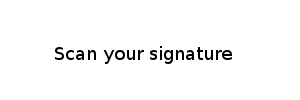
\includegraphics[height=1.5cm]{images/signature.png}
%
%\vspace{1.5cm}
%
%https://pdfs.semanticscholar.org/d3b8/22adbf854ead63144b9472f37784a5ce52a3.pdf
%
%%%For the supervisor: Please type in your fullname according to the order given and include your electronic signature here%%
%Supervisor: Firstname Middlename Surname 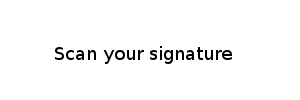
\includegraphics[height=1.5cm]{images/signature1.png}


\newpage

\chapter*{ACKNOWLEDGEMENTS}
%\addcontentsline{toc}{chapter}{Acknowledgements}
% Don't change anything above this.
% We do not number this or add it to the contents!
% Overly long acknowledgements are not professional.

%This is optional and should be at most half a page.
%Thanks Ma, Thanks Pa. One paragraph in normal language is the most respectful.  
%
%Do not use too much bold, any figures, or sign at the bottom.
%\newpage
\chapter*{DEDICATION} 
\addcontentsline{toc}{chapter}{Dedication}

%This is optional.
% Abstracts are usually written in English, with a version in your
% mother tongue underneath
\chapter*{Abstract} 
%\addcontentsline{toc}{chapter}{Abstract}
% Don't change anything above this.

Reports are key source of information for all activities within  organizations. Electronic reports are generated day to day in unstructured way. It is still a big challenge to know automatically what the reports are talking about.  For big organizations like International Federation of Red Cross(IFRC) where they work in humanitarian domain, some information from their reports are quietly necessary and very important. Within million reports, automation of extracting information saves time and increase quality. Needed information from the reports are called Named entities. This research, We used machine learning algorithms such as Stanford NER, polyglot and Natural language toolkit  to extract named entities from IFRC reports. We are looking for the answer of " Who did what when How" from the documents. 


% Don't go typing out the contents.
\tableofcontents
\newpage
% We switch to arabic numerals here where your page count starts
% Essays must be 35 pages long *starting here* and up to and including
% the conclcusion. It does not include the acknowledgements or references.
% 
% Figures may differ between topics, but they are not there
% to fill the pages -- they must add meaning.
% In general most figures should be 0.8 times the width of the page
% (perhaps wider in total when two or three columns of figures)
% See the example in chapter one for defining that. Be *consistent*
% in your presentation of information.
\pagenumbering{arabic}
\pagestyle{myheadings}
%-----------------------------------------------------------------------------
% Each chapter goes in a separate file
% Chapter titles are just examples
% Always have a question
% Note the Case Pattern used at AIMS
\chapter{Introduction of the Research}

%\Jnote{Please read the text again and correct language mistakes. Also pay attention to punctuation.}
In every organization there is a way to communicate. One of the most popular way to transmit the information  is  to produce a written report which explains how different activities of the organization are going. For large organizations there are huge number of reports and it is so challenging to go through  each and every report manually.
%\Jnote{``imagine the way...'' This is not good language for a research essay.}
This research has an aim of providing an easy way of visualizing and extracting the important information locked in reports from NGO and large organisations.

In 1919, the International Federation of Red Cross and Red Crescent societies (IFRC) has been founded, it has some millions of reports related to humanitarian support, How to  know automatically the number of people who suffered from a disease?  How to know the  fraction of fund spent on shelter?  

In this research, we tried to use a combination of statistics formulae  and techniques of Natural Language Processing (NLP) to find the solution for the extracting entities, 
Big data and Machine learning for analysing the huge data by using statistical and computing algorithms. Entity can be defined as an instance of existence of something, for example what is the activity done on what place when and how ?  

Document modelling by extracting entities is one of the way to deal with natural big data linguistic problems where entity can be considered as a single unit of data like location, people, organization and so on. Entities  can be classified based on their relationship.

%\Jnote{Paragraph above has many topics (organizing information, Red Cross,
%  NLP, document modelling) mixed together. Please separate them into
%  paragraphs.}  
These are key procedures to be performed for extracting entities: 
%\Jnote{s/Let .../For example, consider an IFRC report...}
\begin{itemize}
\item The sentences which compose a report  must be parsed.
\item Entities must be identified in the report and classified.
\item Relationship between entities must be modelled.
\end{itemize}

A report is composed by  paragraphs, each paragraph is made by sentences. Natural  Language Processing techniques deal with sentences and content based analysis by splitting the sentences into tokens then remove the common words and work with corpus to get entities. The meaning of a word can depend on its surroundings as well as it can be independent. For extracting significant entities, the context of a word is one of the points to be considered carefully. 
\chapter{Literature review }
In today's life, many organizations are generating unstructured data while they are communicating. There are plenty of entities to be extracted. In this research,  all reports we considered are written in English.

%\Jnote{This is not good english, you can write
 % ``There are plenty of entities to be extracted...''}
%In this research, all reports we considered are written in English.
%\Jnote{Be more specific, e.g.,}
To label the boundaries of sentences is one of the important prerequisite steps in Natural Language Processing. The punctuation marks cause some ambiguity  \citep{baluja2000applying} for example it is challenging to differentiate the point in abbreviations and a full stop. 
To handle this ambiguity some systems use the special purpose-regular expression grammar, exception rule method etc.

David Palmer and Marti A. Hearst worked on the problem of punctuation marks. \citep{palmer1994adaptive}. They developed an efficient system with high accuracy in automatic labelling the boundaries of the sentence  by using the feed forwarding neural-networks where the input was the POS probabilities of all tokens which are surrounding the punctuation  and output was found as the label to be assigned to the token.This work was able to correct up to $98.5\%$ for punctuation of  sentence-boundaries. A proposed  new approach was how to represent the context of punctuation marks without ambiguities.

This research will also look at how neural networks can be used to label different tokens.

Capitalization can be used in different ways such as the beginning of the proper noun, the abbreviation, the post of high level profile people etc. Considering the English language text, if we are given a  particular token it is not by chance  to  determine whether it is a name or not. Some of the approaches to indicate a name are to  use capitalization, detection of sentence boundaries and dictionaries \citep{baluja2000applying}.

%\Jnote{Consider putting text above into separate section (preprocessing for NLP).} 
\section{ Parse  Tree} \label{tree}
One of the sentences that compose our sample report says: 
"Assessment reports indicated 117 deaths, 544 people injured, 12,794 homes damaged and 7,384 houses destroyed", Suppose that this sentence is called "S"

There are two mains steps which can be performed to get the entities from  this sentence:
\begin{itemize}
\item \textbf{Tokenizing}: This is a procedure of taking a sentence and extract the composing atomic linguistic elements e.i. words, verbs, punctuations, adjectives etc .
S has the following tokens: ['Assessment', 'reports', 'indicated', '117', 'deaths', ',', '544', 'people', 'injured', ',', '12,794', 'homes', 'damaged', 'and', '7,384', 'houses', 'destroyed']
\item \textbf{POS}: part-of-speech is a process of attaching to every linguistic element of the sentence a corresponding tagg based on grammar rules.
The POS of S  are: 
[('Assessment', 'JJ'), ('reports', 'NNS'), ('indicated', 'VBD'), ('117', 'CD'), ('deaths', 'NNS'), (',', ','), ('544', 'CD'), ('people', 'NNS'), ('injured', 'VBN'), (',', ','), ('12,794', 'CD'), ('homes', 'NNS'), ('damaged', 'VBN'), ('and', 'CC'), ('7,384', 'CD'), ('houses', 'NNS'), ('destroyed', 'VBD')]

The meanings of the used tags for S:
\end{itemize}
\begin{itemize}
\item JJ: \textbf{Adjective}: 'Assessment'   
\item NNS: \textbf{Noun, plural}: 'reports', 'deaths', 'people','houses'
\item VBD: \textbf{Verbs, past tense}: 'indicated',             'injured', 'damaged', 'destroyed'
\item CD: \textbf{Cardinal Number}: '117', '544' '12,794','7,384',
\item CC: \textbf{Coordinate Conjugation}: 'and'
\end{itemize}
%\Jnote{Can you give a citation for this method?}
The parse tree is formed based on the POS, the classification of word and the way words are arranged in a sentence show a kind of relationship between words.
\begin{figure}[hbtp]
\caption{Relations extraction from }
\centering
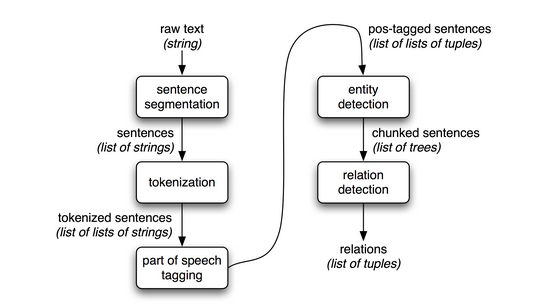
\includegraphics[scale=0.7]{images/nltk.png}
\end{figure}



\section{ Named Entity Recognation and Classification  NERC}
%\Jnote{Please do not number sections by hand.}
The term "Named entity" has been coined in 1996 in "sixth  Message understanding Conference"(MUC-6  R. Grishman and  Sundheim 1996).
%\Jnote{No manual citations, use \textbackslash cite in LaTeX. Also it is not usual to write the conference name, just {``has been coined in 1996 by \textbackslash cite{\}''}
Entity can be referred as a task, the entity is "named" when it is restricted to one or many rigid designators \citep{sharnagat2014named}, example: persons, location, product are the named entities.

Based on the classification of Standard Generalizes Markup Language (SGML) a task can be divided into three subtasks:
\begin{enumerate}
\item ENAMEX: location,product,country ,organization
\item NUMEX : percentage,quantity 
\item TIMEX : time, date
\end{enumerate}


The entities from different reports.
For extracting entities in a report there are different models which can be used:

\section{Hidden Markov Model}
This model is based on Bayesian probability inference which has been initiated in 18th century. HMM is the earliest applied model for Natural Entities Recognition for English language.The way to perform these tasks is to find the most likely sequence of tagged names(TN) given a sequence of words(SW).
\begin{align}
P(TN|SW) & = \frac{P(SW|TN)P(TN)}{P(SW)}\label{eq2.0.1}
\end{align}
The equation  \eqref{eq2.0.1} is conditional probability, $P(TN|SW)$ can be  called posterior and it is  the probability of an event Sequence of word occurring given Tagged names has observed. 
$P(SW|TN)$ is also called likelihood e.i.  it is the probability of observing the sequence of words(SW) when the given hypothesis tagged name (TN) is true. On another hand P(TN) doesn’t depend on the evidences, P(TN) is called prior e.i.  that it is true even if there is no given evidence at all(masters thesis). We can be ignored P(SW) and the remaining objective is to maximise the probability of getting the sequence of tagged names when sequence of words is given.
%\Jnote{``The above sentence is true.'' Delete that.}
%\Jnote{s/there is a permission to say/we can ignore}
%\Jnote{s/remaining purpose/remaining objective}
\begin{align}
Max\left[P(TN|SW)\right] \label{eq2.0.2}
\end{align}
From the equation \eqref{eq2.0.2} of the maximization, the following estimation can be made.
\begin{align}
P(TN){\approx} \prod_{i=1}^{n} P({TN}_{i}|{TN}_{i-1})\label{2.0.3}
\end{align}
Where ${TN}_{i}$ is a tag in the sequence of names (TN), for the likelihood probability can be estimated as :
\begin{align}
P(SW|TN){\approx}\prod_{i=1}^{n} P({SW}_{i}|{TN}_{i})\label{2.0.4}
\end{align}
%\Jnote{There is a typo in formula above.
%  Try explaining better what those estimates mean, something like
%  ``we make a simplifying assumption that the tags occur independently
%  from each other''.}
The above estimations was for a small sequence where ${TN}_{i}$ is a tag in the sequence of names (TN) and ${SW}_{i}$ is a tag at index i in a sequence words (SW). For the large training corpus, the needed step is estimate based on the number of times the tag occurs and the position of the tag in a given corpus.
\begin{align}
P(T_{i}|T_{i-1}) = \frac{K(T_{i-1},T_{i})}{K(T_{i-1})}\label{2.0.5}
\end{align}
Based on the training corpus, $K(T_{i-1},T_{i})$ is referred as a how many times the tag $T_{i}$ occurs after the tag $T_{i-1}$. In the corpus, $K(T_{i-1})$ is considered as the number of occurrences for the tag $T_{i-1}$.

Therefore the estimation can be performed as follow:
\begin{align}
P(C_{i}|T_{i}) =  \frac{K(T_{i},C_{i})}{K(T_{i})} \label{2.0.6}
\end{align}
From the equation \eqref{2.0.6}, the term $K(T_{i},C_{i})$  is referred as the sum of the times that a word "$C_{i}$" has a tag $T_{i}$in the training corpus.
The process of computing the posterior using the above steps is called Markov model.

%\Jnote{This is a beginning of a good explanation, but you need to rewrite to correct language mistakes and clarify some points.}

%\section*{2.1.1.1. Advantages of Hidden Markov Model}
%\Jnote{There is no need for a separate section, just put it in another   paragraph.}
It is one of the most powerful statistical and machine learning (ML) techniques in modelling and high qualified in entities extraction. When the researcher is willing to train new data, HMM is very robust and efficient in computations.
%\section{2.1.1.2. Disadvantages of Hidden Markov Model}
One of the limitations of HMM is that the researcher must have the notion of model topology and statistical techniques on how to deal with large amount of training data.
\section{Supporting Vector Machine (SVM) based model}
This model has an aim of classifying the named entities by separating the documents into two categories.  The document must belong to one category, either positive or negative.  SVM can classify linear data as well as non linear with a purpose of maximizing the margin between negative and positive documents.The plane which separate those two categories is called "hyperplane".

The main idea behind SVM modelling is to work with features and find the hyperplane. The hyperplane must separate all given samples regardless the dimensions.
\subsection{Linear Supporting Vector Machine }
\newpage
\begin{figure}
        \begin{subfigure}{.6\textwidth}
         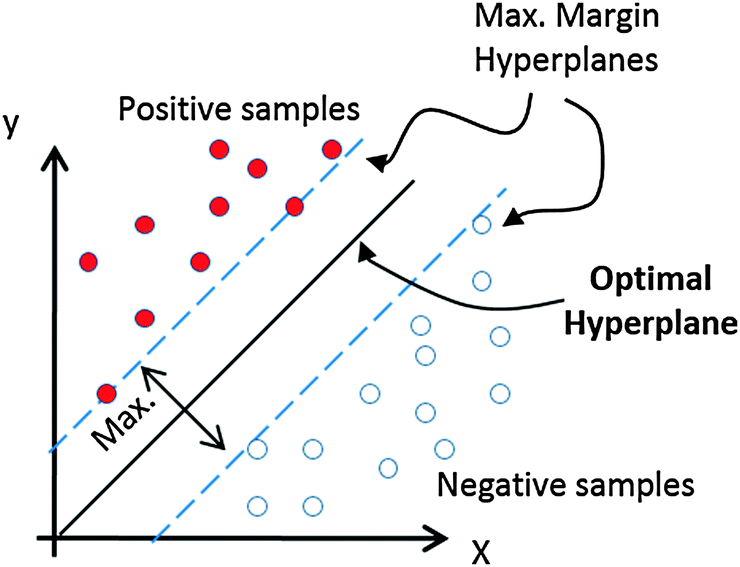
\includegraphics[scale=.3]    	          {images/linear.png} \label{linear}
         \caption{Two dimensional SVM}
        \end{subfigure}%
        \begin{subfigure}{\textwidth}
                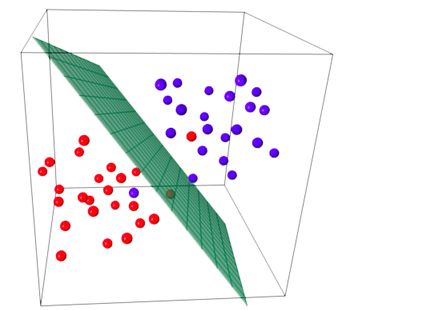
\includegraphics[scale=.6]    	                 {images/multi.png}
                \label{multi}
                \caption{Multi dimensional  }
        \end{subfigure}

\end{figure}
For linear sample data, it is simple to plot the hyperplane to handle the separation.  Data are spread separately between positive documents and negative documents. The way data are represented SVM decided  whether to use linear modelling or not. IFRC reports are considered as multi dimensional documents.

\subsection{Non Linear data} 
Sometimes the representation of data is quite mixed way so that you cant plot hyperplane easily. When the hyperplane can not be plotted as a straight line,  SVM has a function to linearise non linear data.  When the data are not linear, SVM has a way to linearise them by using a function. $ \phi$ maps data to the higher dimensional space. Straightforwardly, the classification became linear. Figure \ref{SVMNL} shows the way a function $ \phi$ linearised the data.

\begin{figure}[hbtp]
\caption{Nonlinear SVM classification}
\centering
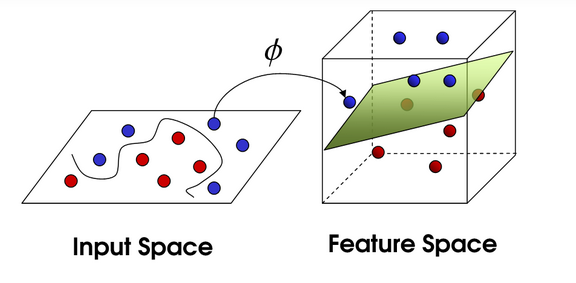
\includegraphics[scale=.7]{images/SVMNL.png}\label{SVMNL}
\end{figure}
 
\section{Disadvantages of SVM} 
The classification of particular documents is not easy to be performed by SVM without destroying the constructed weights  but with hand-written rule model. Machine learning uses decision tree procedure than SVM. In addition the decision tree has a detailed boolean-like  model which is more popular to user.

\section{Some Terminologies}

\textit{Hand-written rule}

It is one of the standard approaches of NER and IE, it has been used for extracting the patterns from automated pages such as amazon, NLP is so useful for unstructured humman-written text by delivering  part-of-speech (POS), syntactic parsing and categories of semantic words.

\textit{Rule /pattern based extraction}

Many IE systems uses rule/pattern to extract words and also phrases by looking to the context of those words or based on the their surroundings.\citep{califf2003bottom}. Some system decided if the procedure of extracting the words should rely on the meaning of each word independently or on the context of their surroundings in a phrase.
The limitation of this method is that some words do not have a closer mining to their surroundings that is why Patwardhan Siddharth with help of Ellen Rilo  in workshop called "ACL 2006" presented another approach which  was  generating an automated IE system to learn patterns from a large fixed data set  within a specific domain \citep{patwardhan2007effective} 

\textit{Bag of Words} 

It is referred to the multi-set of words represented by Natural Language Processing and Information Retrieval(IR). They are used  for classifying the documents.

Our research deals with reports generated through a template, compared to the work of  \citep{patwardhan2007effective} templates usages is a limitation.

\section{Text classification and Naive Bayes}


It is one of the most important algorithm in text classification by using base rule and bag of words to classify the entities \citep{manning2012information}.The user instead of going through the report and start posing many queries, text classification algorithm transient the need information.
Its aims is to build a function $\theta$ which takes the bag of words and returns the class of sentiment $C$ either positive or negative.
\newpage
{\centering{$\theta$}

\centering{$\Updownarrow$}   

\begin{figure}[hbtp]
%\caption{a part of a sample reeport}
\centering
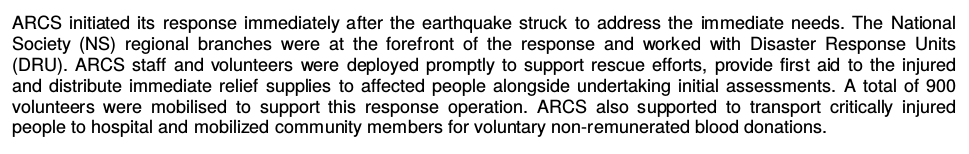
\includegraphics[scale=0.4]{images/report.png}\label{report}
\end{figure}

{\centering{$\Updownarrow$}}

{\centering{C}}

The procedure is to look for all words and retrieve those which form the subsets.  Bag of words are formed after throwing away  all words except the subsets.The use of the function $\theta$  is for  attributing  to each item of the bag of words a sentiment.}

\section{Machine learning for Named Entities\label{Chapter2}}
The natural language processing is not enough to handle the sophistication and ubiquity of textual data. Deep learning using machine learning techniques has been introduced to solve this problems. The advantages of machine learning for Named Entities:
\begin{itemize}
\item Manual extraction of entities is too expensive.
\item Fast processes of extraction.
\item extraction done by learning algorithms and Natural language tools.
\item No limitation of languages.
\end{itemize}


  
\chapter{Research Methodology}
%\chapter{Research methodology}
\section{Data and tools}
World wide non governmental organizations publish some of their reports on their official websites.  Web scrapping is one of the ways to extract data from website to the local machines. We downloaded the reports about appeals in pdf format from IFRC website. 
 We used R-scripts for web scraping form our co-supervisor professor Xavier. 
 
 
We downloaded 1262 reports which have been submitted between $ 1^{st}$ January 2015 and $31^{st}$ December 2016. To differentiate the reports, each report has  a report Id but different reports can refer to the same appeal Id.
As an international organization which insights on the largest humanitarian  activities in the world, IFRC reports we have talk about disasters and cash transfer program.
Cash Transfer Program (CTP) describes the money used by IFRC to buy food, shelter, etc.
\section{Data Analysis and Filtering}
Portable document format (PDF) has content which can not be extracted and manipulated  easily. The data we have has to be changed into another format in order to pull the information we need. We managed to transform 1260 reports.  Our folder has the 1260 $ txt $ files which is considered as dataset. For analysing the data, we used  python programming language.

Our data reported on different areas of the World such as continents, countries and cities. For example "Europe IB23102015 23Oct2015.txt" covers European continent , "Afghanistan MDRAF003 05Nov2015.txt" and  "Japan 0 16Apr2016.txt" reported  on specific countries and  "Port au Prince country cluster 0 04Oct2016.txt" reported on the most popular city of Haiti.
-
\section{Supervised vs Unsupervised  Machine Learning}
\begin{itemize}
\item \textbf{Supervised} is a machine learning part which deals with "labelled data",  data are categorized and classified. We have a csv document which summarize the appeals what we have. The shape of this document is 25 columns and 3997 rows. The "CTP" feature indicate if the appeal is classified as a Cash
Transfer Program document  or not. Among 3997 appeals, 404 are CTP. 

\item \textbf{Unsupervised} can be defined as a way machine learning processes ”unlabelled data”.
the data are unstructured, uncategorised and unclassified. The reports we have are good example of unlabelled data.
\begin{itemize}
\item clustering is a technique for analysing data by identifying hidden groups in a data set. The hidden groups helps the machine to  classify them data into small groups called "cluster" based on similarities or relationship found in data \citep{dy2004feature}.
\end{itemize}
Unsupervised Machine Learning is very important, the analysis of data require the machine to use its brain Supervised learning.
\section{NLP Corpus}\label{re}
%Corpus is a set of large data which are structured and                                                                                                                                                                                                                   
%\section{CORPUS}
Corpus is a set of large data which are semi-structured.  To extract entities from corpus is simple than to deal with unstructured data. To get the corpus we filtered the data by using unicode of utf-8.

To get compatible data, we have to filter using the Unicode provides canonical and compatible equivalence.


\textbf{Regular Expressions}: in Python, regular expression has operations and modules like "re.py" aND so on. they are used to manipulate characters in strings. regular expressions use a backslash $(" \backslash  ")$  to indicate a special form without invoking the meaning of the special form. There are many regular expressions functions but some of what we used the most are :
\begin{itemize}
\item re.split(): this function split par pattern and return the list of string.
\item re.search(): it returns match objects.
\item the match object ".end()": in a search string, it returns the end position of the match.
\item the match object: in a search string, it returns the start position of the match.
\end{itemize}

\textbf{ASCII} stands for American Standard Code for Information Interchange. it is uses numbers to represent text by using 128 characters. Computer uses ASCII exist within unicode for storing texts easily. All  ASCII uses unicode. ASCII characters are used to send and receive the e-mails, for text files and data conversions. 


\begin{itemize}
\item  ASCII-encoder: transform text to numbers.
\item  ASCII-decoder: transform numbers to text.
\end{itemize}
\newpage
\begin{figure}[hbtp]
\caption{ASCII TABLE}
\centering
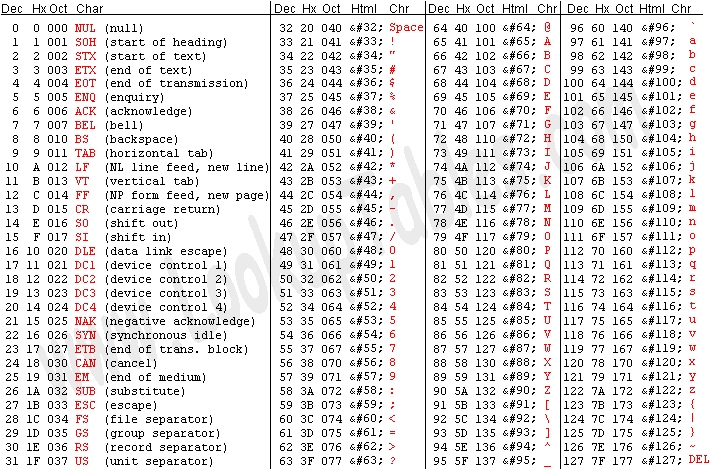
\includegraphics[scale=.5]{images/ASCII.png}\label{ASCII}
\end{figure}
\end{itemize}
%\end{itemize}

Figure \ref{ASCII} demonstrates Unicode  standard. It provides  a unique number to each character composing a text regardless the language, program  or platform.
UTF stands for Unicode Transformation Format. Unicode characters are set into binary values 0 and 1. UTF-8 for encoding  8 bytes, UTF-16 for encoding 16 bytes and UTF-32 which is a standard for encoding 32-bytes are three current standards.
For our corpus we used UTF-8.

After getting semi-structured documents, we removed the StopWords which are defined as unnecessary words for extraction of entities from corpus.

Normally the StopWords return vast amount of unwanted information. Some example of English Stop Words: almost, are, or,  details, during, upon and so on.

Now we can check how for all of 1260 documents and count the Stop Words to be removed from vocabularies of corpus. We trained corpus by nltk package called FreqDist which uses  frequency distribution of each word occurs in corpus, then the module of nltk technique called "nltk.corpus.PlaintextCorpusReader" helped us to get total 58104 stop words over the whole  7796263  vocabularies.

\section{Modules and packages}
The procedure of extracting entities requires many linguistic packages. Machine learning algorithms check grammar rules, punctuation marks and syntaxes. For some    research eras ,  documents can have special characters such as emoticons for emotions. To install these package, you must understand clearly how they work and the content type of your documents. This is a list of packages we used for extracting IFRC entities.
\begin{itemize}
\item \textbf{os} : This module is  known as miscellaneous operating system interfaces. os represents the functionality of operating system with independent functions such as os.path.isfile(), os.path.exist, os.path.isdir, etc.  

Its functions are important for building andependant platform. The programmes written  using os module  can execute in Windows and Linux regardless the machine operating system. 

\item \textbf{nltk}: Natural Language Toolkit is one of core packages for linguistic modelling . With various important  built-in functions nltk is able to manipulate documents.  The main idea behind nltk is to use $nltk_{-}corpus$ to collect all documents as one dataset, then split the documents into sentences using $ne_{-}chunk$ and  remove the stopwords by  importing $stopword$ from $ntk.corpus$, lastly apply machine learning algorithms to extract entities.

\item \textbf{PyPDF2} is able to extract specific information from a pdf document based on the section they belong to. This package locates top section, title, author, etc. It has many functions such as splitting documents pages, merge document pages, encrypt and decrypt documents and so on. It can be compared to pdftk
\item \textbf{pandas} is an open source with high performance structure within various build in functions.
Dataframe design for presenting many data in organized way. Pandas is powerfull in data analysis, flexible, fast and manipulation took for any language. In our research, We used pandas for making the frames of our data.
\item \textbf{codecs} module  offers unicode string for encoding and decoding. codecs is used for handling errors and gives freedom to access internal registry. Codecs are not limited to text but mostly are for text encodings which is for encoding text to bytes. Additionally, there exits codecs for encoding text to text, some codecs can encode and decode at the same time.
\item  \textbf{defaultdictionary} has basic content of difference between verbs, nouns, adjectives, adverbs etc. It uses tagger to assign each word composes the sentence a corresponding POS as explained in Chapter \ref{tree} classes of words are inverted by NLP, it refers to categories of words in dictionary.
\item \textbf{Python String} module which returns a string with trailing text removed.  It has two methods to strip text on both sides, right strip() and left strip(). Trailling text can be  unwanted space, extension, punctuation marks, etc.

To indicate the position of the character to be stripped we use left(l.strip()) which removes the character at the beginning of a string or right(r.strip()) to remove the character at the end of the string.
\item \textbf{regular expressions } regex is a module which finds out the patterns between strings by setting rules for text. bytecodes compile those pattern rules and execute using matching rules.  example methods for re are explained into Chapter \ref{re}
\item \textbf{polyglot} is used to extract entities from many languages.  It is multilanguage application supporter built as natular language pepeline.
\item \textbf{Stanford} is one of most brilliant algorithms to extract entities from  documents corpus. it has classifier models, jar files which are free downloads. Stanford has many packages to handle linguistic problems. 
\end{itemize}

\section{Extraction of Entities }

To extract entities we used default dictionary built in collection package of nltk. Our dataset now is a folder containing 1260 corpus files, we  used nltk chruncker to get sets of sentences of corpus. let have a look for our sample document the way sentences are split. 
\begin{figure}[hbtp]
\caption{Set of sentences}
\centering
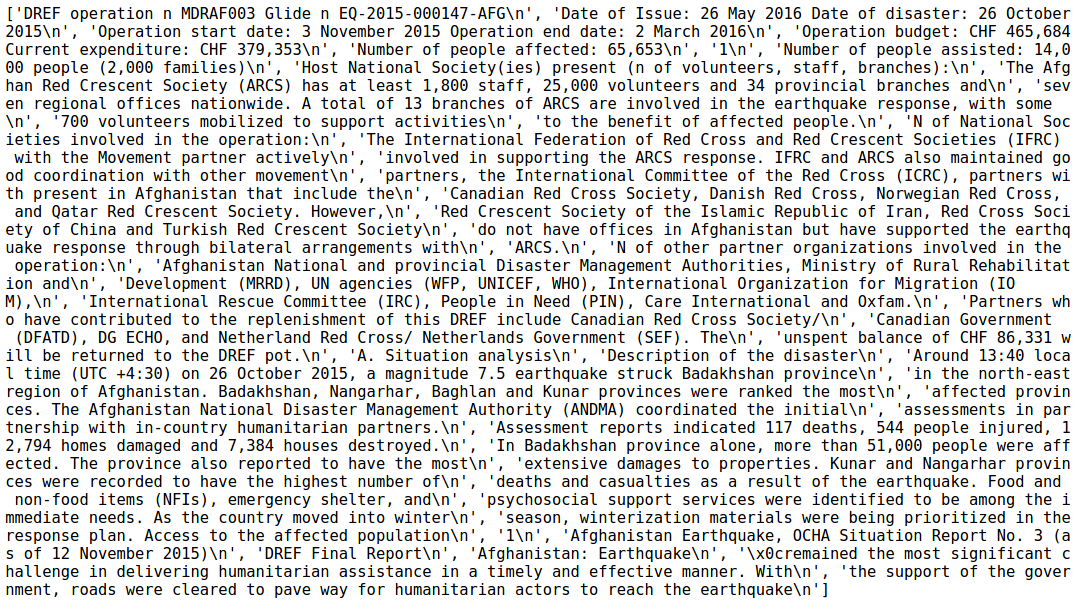
\includegraphics[scale=0.4]{images/corpus.png}\label{Set of sentences}
\end{figure}


Figure \ref{Set of sentences} shows the 45 first lines of the sample document. each each line is ended by  $'\backslash n'$. 

\section{Top Section Dataset \label{top}}

From the analysis of IFRC pdf reports, most of them have a small table on the top. this table gives the image of what the report is talking about. This table summarizes what the document is talking about. For example the total amount of money spent in recovering a disease, the number of people who participated in a given activity, the location and so on.

While we were transforming the pdf data into txt format, this table occupied almost 25 first lines. Due to the limited time of the research, We decided to split those twenty five first lines of each document. the collection of those first twenty five documents has been considered as our new corpus.

Now  we can use  one of the algorithms to extract entities and for classification.

\section{Stanford Named Entities Recognition}

The data to be trained is unlabelled. Named Entities Recognizer labels the data to be extracted easily. it recognises sequence of words and its classification is mainly to name of persons, localization and organization.

Stanford Named Entities Recognition is an extractor implemented in java. It takes the sequence of words and label them 
Stanford named entities recognition is  a able to identify correctly the named recogniser which labels sequences of words in a text. The next step is to split the sentences into set of words called tokens. By using the Stanford NER tokenizer  where token can be tagged. 

\begin{itemize} 
\item \textbf{Stanford NER Tagger} is a package which has modules for classifying tokens with the taggs. A tagg can be defined as one of classes of significant words like nouns, adjectives etc. we used the package Stanford POS Tagger to classify the words. 
\item \textbf{Stanford NER Models} are many Stanford has different models such as "stanford-corenlp-full-2016-10-31", "stanford-ner-2014-01-04" which is the version we used. 

\item \textbf{Stanford Classifier} is a package which classify the entities into defined categories. It has four specific classes such as  "Locations",  "Persons",  "Organizations" and    "Others".
\end{itemize}

We specified the named entities that we wanted to extract. We classified them into the four categories by Stanford classifier.  The last category called "others" combined all numerical entities such as time, amount of money, number of people, percentage, etc. 

The reports from our corps are order by appeal numbers, the entities are in classified by nltk algorithm. 

\newpage

\begin{figure}[hbtp]
\caption{IFRC entities from Stanford NER}
\centering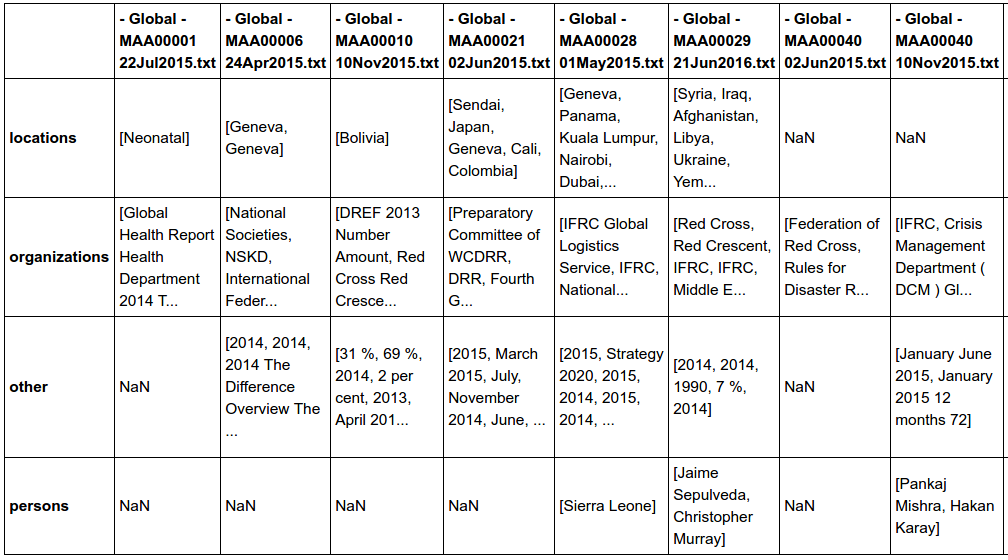
\includegraphics[scale =.45]{images/stanford.png} \label{stanford}
\end{figure}
From Figure \ref{stanford},  Consider the for the report "-Global MAA00029 21Jun2016.txt", locations row  shows that the report covered Syria, Irak, Afganistan, Libia, Ukraine, Yemen, etc.
The extraction of entities separates clearly the categories.
\section{Natural Language ToolKit (NLTK)}
Natural language toolkit is one of the algorithm to extract named  entities. It has different modules which are used to process the data alongside the extraction.
NLTK chunkparser is a one of nltk module  which uses Regular expressions. NLTK tokenize which splits the sentences into small units called tokens. This module helps the NLTK tagger to identify words independently. 

Generally NLTK classify the entities into four categories which are known as Location, Organization, Persons and Others. 
\newpage

\begin{figure}[hbtp]
\caption{IFRC entities from NLTK}
\centering
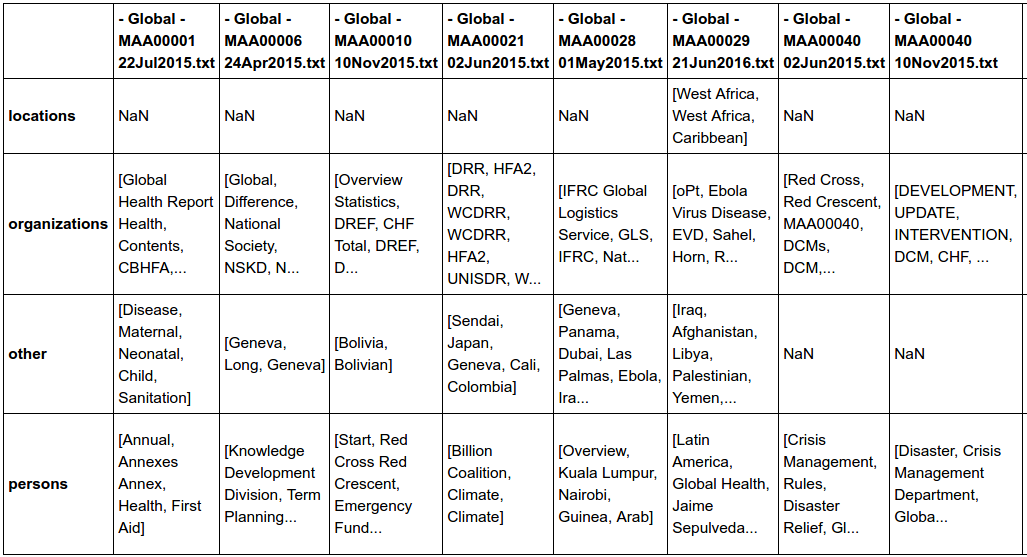
\includegraphics[scale=.45]{images/nltkalgo.png}\label{nltkalgo}
\end{figure}

From Figure \ref{nltkalgo}, Consider organizations extracted from the report "-Global-MAA00021 02 Jun 2015.txt", NLTK entities classifier was able to extract DRR, HFAR, WCDRR, HFAR2, UNISDR, etc. The classifier uses nltk tagger and default dictionary which help it to identify the names, verbs and adjectives.

\section{Polyglot Named classifier}

Compared to previous entities extractor, Polyglot has only three categories which are "Persons", "Locations" and "Organizations". For nltk, any entity which is classified into those three categories is not considered as named.
\newpage

\begin{figure}[hbtp]
\caption{IFRC entities from Polyglot}
\centering
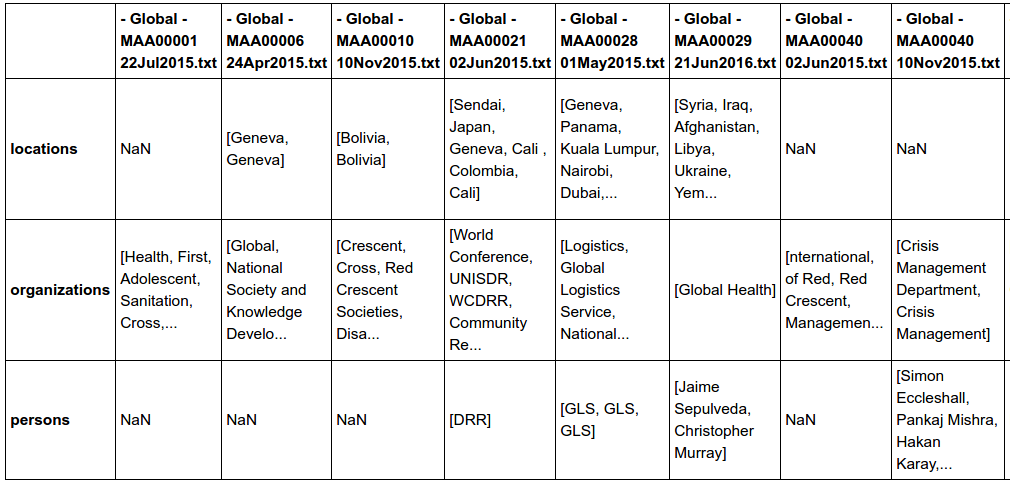
\includegraphics[scale=.45]{images/polyglot.png}\label{polyglot}
\end{figure}
Let us take an example report "-Global-MAA000029 21 Jun 2016.txt" from Figure \ref{polyglot}, the entities which are classified as "Persons" Jaime, Sepulveda and  Christoper Murray.




\section{Sample Files} 
The type of data we have can be considered into two different ways. There are some reports which are classified as CTP documents. This documents cover the overview of how IFRC money was invested in humanitarian activities.

Non CTP reports are focused on other activities which didnt require IFRC to invest money. 

The next step is to take example report document for CTP and Non-CTP to have a comparison on the extracted entities.  







































%\section{Entities Recognition and Classification}
%%\newpage
%\begin{figure}
%        \begin{subfigure}{0.5\textwidth}
%         \caption{Organizations sample}
%                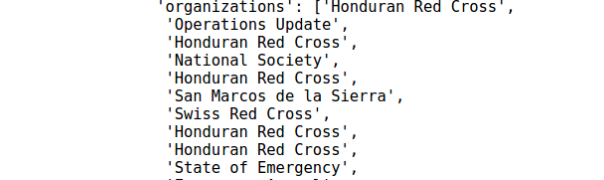
\includegraphics[width=\textwidth]{images/organizations.png}
%                \label{Organizations}
%        \end{subfigure}%
%        \begin{subfigure}{0.5\textwidth}
%        \caption{Location sample}
%                
\includegraphics[width=\textwidth]{images/location.png}
%                \label{Location}
%        \end{subfigure}\\
%        \begin{subfigure}{0.5\textwidth}
%         \caption{Person's names}
%                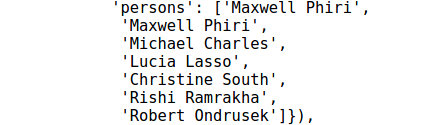
\includegraphics[width=\textwidth]{images/person.png}
%                \label{Persons}
%        \end{subfigure}%
%        \begin{subfigure}{0.5\textwidth}
%        \caption{Others category}
%                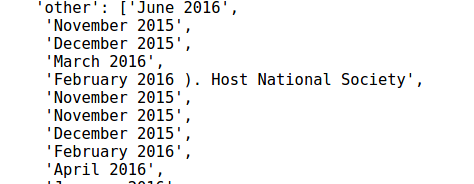
\includegraphics[width=\textwidth]{images/others.png}
%                \label{Others}
%        \end{subfigure}
%\end{figure}
%
%\section{Entities linking}
%Natural languages used by human are inherently noisy, spelling mistakes and ungrammatical mistakes. Machine learning algorithms are able to handle linguistic problems.  
%\section{Context}
%\section{Bag of words}

%
%
%The frequency of a word is calculated based on summation of times the word appeared into a document. The frequency is used in words classifiers.
%
%\section{Mathematics behind entities extraction}
%\section{Supervised Classification}
%They are key points to classify the data which are supervised:
%
%\section{Corpus from Natural Languague Tolkit}

%The check-up on the entities extracted from the text can be done by comparing what has been extracted by hands and what the algorithm give us as results.

%The check-up on the entities extracted from the text can be done by comparing what has been extracted by hands and what the algorithm give us as results.
         
\chapter{Results Discussion and Testing}
\section{General Overview}
To extract and classify entities, We used Stanford, NLTK and Polyglot. These entities extractor have common categories which are "Persons", "Location" and "Organization", Additionally NLTK and Stanford NER has another category which is called "others". This last category is not very clear. It combines numbers, percentage and unclassified entities. This can cause the confusion for to the organization. The core categories are those three first groups.

Among these three entities extractor, Stanford requires time to run compared to others.

The named entities must be setted by the organization based on its interest. Some reports are composed by many pages but some few point must be highlighted. Templates in reporting are important, they made life easy.

Before extracting the entities, You must know what the document is  talking about. What the organization is struggling to know from the report.


Named entities from NLTK, Polyglot and Stanford are useful. They tried to summarise the primary information such as locations, persons and organizations. 

Sometimes, extracted named entities are not sufficient. You can  used Regular expressions to respond perfected the will of the organization.

\section{Case Study Results}
After analysing 1260 documents, Let us take one sample file and work on top section composed by 25 lines.

Consider a document which is specific to African region. "Africa regional office MDR60002 03 Nov2015.txt". We are requested to extract name of Persons who participated in IFRC activities.

We had a function to extract four categories of entities by Stanford NER. It is only to specify the category we are interested in. To identify persons names manually is also possible.
%\subsection{Stanford NER}
%\subsection{Polyglot}
%\subsection{Stanford}

\newpage
\section{Testing}\label{chp4}
For the security purpose testing gives a guarantee of correctness.  It is a major chapter for assertion of the research quality. Typically our research is a part of big data and Machine learning. We used analysis and statistical testing to make sure that the results are true.

The process of extracting entities can be done in different ways. Either manually or by the use of machine learning algorithms. The manual way has many disadvantages as explained in Chapter \ref{Chapter2}.

Computer algorithms have impact for solving human problems. However we have to do a comparison for a small dataset between algorithm results and human results. The correctness of a tested dataset gives a confidence for remaining datasets.

IFRC uses the templates formats to produce their report. It is way of structuring a content of the document. The use of templates made most IFRC reports to have almost  the same size of top section. Top section contains important summary  as explained in Chapter \ref{top} .

Due to the time limitations, We tested  some  sample documents and We concluded for all top sections of the reports.
\section*{JSON file }
By taking the sample file, We extracted names of entities in JSON format. JSON stands for Java Script Object Notation. It is built based on two universal data structures such as a pair composed by a name and a value, and ordered list of values which is considered as an array, sequence, vector or list.
\begin{figure}[hbtp]
\caption{JSON File Structure}
\centering
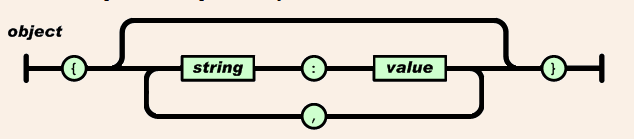
\includegraphics[scale=.7]{images/json.png}\label{json}
\end{figure}


Figure \ref{json} refers to the structure of our json file. It contains a small dictionary which has one feature of proper names. We are able to identify three people who participate in IFRC sample report.
\newpage 
\begin{figure}[hbtp]
\centering
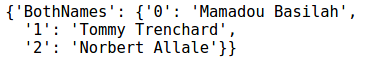
\includegraphics[scale=.7]{images/BothNames.png}
\caption{Persons Names Extracted by Hands}\label{Hand}
\end{figure}

After extracting three proper names as the Figure \ref{Hand} shows,  We are now going to do a comparison. We can compare the output of the algorithms.

\begin{figure}[hbtp]
\caption{Comparasion}
\centering
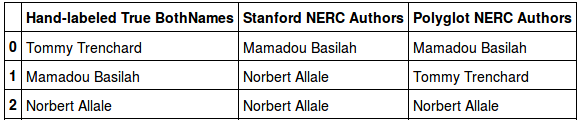
\includegraphics[scale=.8]{images/comparason.png}
\end{figure}


In Machine Learning, there are three ways of testing the quality of algorithms. As We extracted  entities from IFRC reports, to be sure on the work of algorithms,  We calculated recall, precision and accuracy. 

\textbf{Precision} has been calculated as a  fraction of relevant instances over  retrieved instances.

\textbf{Recall} has been gotten as a fraction of retrieved relevant instances over  sum of relevant instances.

%\textbf{Accuracy}

%\textbf{Accuracy}

Prediction is made by algorithms to predict the name of persons in sample document. The correctness can be calculated based on comparison between what predicted and what extracted by hands. The figure \ref{prediction} is  the results of comparison between Polyglot names of 
\begin{figure}[hbtp]
\caption{Precision}
\centering
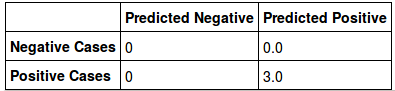
\includegraphics[scale=1]{images/precision.png}\label{prediction}
\end{figure}
 

\chapter{Conclusion and Future work}
Entities extraction has been performed using natural language toolkit, polyglot and Stanford named entity recognition.
Evaluation of entity extraction is normally done by the metrics of precision, accuracy and recall between algorithms and named extracted by human hands.  This research argues that top section of report has meaningful metrics. The results demonstrate that a process of extracting names of persons in top section of reports was well done.

As future work, the next step for entity extraction  is to work on other sections of a document.  To combine all used approaches into a software which can automatically visualised entity named by organization such as budget, number of people suffered from a disaster e 
% Acknowledgements and References are not counted.
%-----------------------------------------------------------------------------
% Note the errata page is not for now, it is for use during the examination.
% Not that you're going to have any errata.
%-----------------------------------------------------------------------------
% THE BIBLIOGRAPHY 
% Bibliography styles define how the bibliography is 
% listed and formatted. This is part of the AIMS house
% style and is only changed under exceptional circumstances
\renewcommand{\bibname}{References}
\nocite{*}
\bibliographystyle{plainnat}
\bibliography{references}
\addcontentsline{toc}{chapter}{References}
%-----------------------------------------------------------------------------
\end{document}
